\section{The Controversy}
\begin{frame}{\enquote{Evidence for neutrinoless double beta decay}}
	\begin{itemize}
		\item 2001-12-05 \emph{part} of the Heidelberg-Moscow collaboration: \fullcite{Klapdor-Kleingrothaus:2001}
		\item Data: \SI{54.98}{\kilo\gram\year}
		\item Claim: Mesurement of $0\nu\beta\beta$ at $2.2\sigma/3.1\sigma\Rightarrow T_{\sfrac{1}{2}}^{0\nu}=\SIrange[scientific-notation = fixed, fixed-exponent = 25]{0.8e25}{18.3e25}{\year} (\SI{95}{\percent}\  \symup{C.I.})$
	\end{itemize}
	\centering
	\only<1>{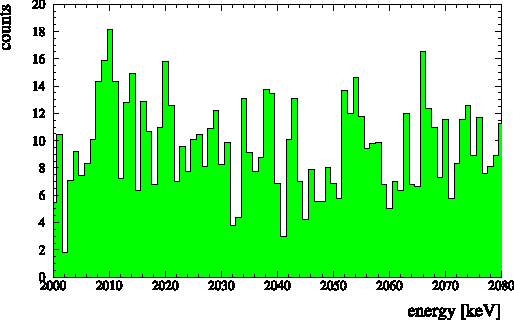
\includegraphics[width=0.5\linewidth]{media/hm_data.pdf}}
	\only<2>{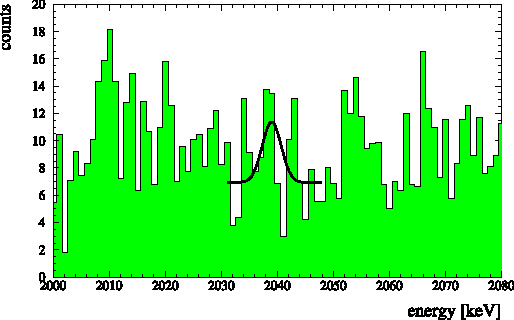
\includegraphics[width=0.5\linewidth]{media/hm_data_peak.pdf}}
\end{frame}
\begin{frame}{\enquote{Evidence for neutrinoless double beta decay}}
	\begin{figure}[htpb]
		\centering
		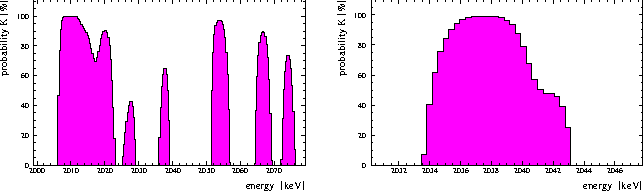
\includegraphics[width=\textwidth]{media/hm_prob.pdf}
		\caption*{Probabiliy of a peak at given position (Bayesian inference)}%
	\end{figure}
	\vspace{-1em}
	\pause
	\enquote{\footnotesize On the left-hand side of Figs. 5,6,6, the background intensity $(1-\eta)$ identified
		by the Bayesian procedure is too high because the procedure averages
		the background over all the spectrum (including lines) except for the line it is
		trying to single out. Therefore on the right-hand side of Figs. 4,5,6, the peak
		detection procedure is carried out within an energy interval that does not contain
		(according to the left-hand side) lines other than the one at $Q_{ββ}$.}
\end{frame}
\begin{frame}{Some Problems of the 2001 Paper}
	\vspace{-0.5em}
	In 2002 two independent papers\footnote{\fullcite{aalseth2002comment}}\footnote{\fullcite{FERUGLIO2002345}} criticized H. V. Klapdor-Kleingrothaus et al.
	\vspace{-0.5em}
	\begin{columns}
		\begin{column}{.5\textwidth}
			\begin{itemize}
				\centering
				\item No Monte Carlo simulation
				\item Unidentified Peaks
			\end{itemize}
			\begin{figure}
				\centering
				\begin{tikzpicture}
					\node[anchor=south west,inner sep=0] at (0,0) {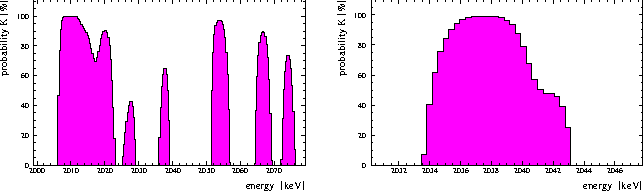
\includegraphics[trim=0 0 150 0,clip,width=\textwidth]{media/hm_prob.pdf}};
					\node at (1.5, 4.05) {$\downarrow$};
					\node at (2, 3.7) {$\downarrow$};
					\node at (2.35, 3.8) {$\downarrow$};
					\node at (4.85, 4.05) {$\downarrow$};
					\node at (5.85, 3.8) {?};
					\node at (6.4, 3.25) {?};
					\node at (2.9, 2.25) {?};
					\node at (3.5, 3) {$0\nu\beta\beta$};
				\end{tikzpicture}
				\vspace{-3em}
				\caption*{${}^{214}\symup{Bi}$ Peaks ($\downarrow$)}
				\vspace{1em}
			\end{figure}
		\end{column}
		\begin{column}{.5\textwidth}
			\begin{itemize}
				\centering
				\item No model testing
				\item Choice of the window
			\end{itemize}
			\begin{figure}
				\centering
				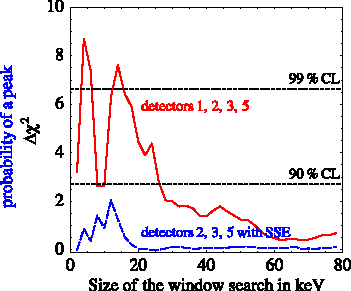
\includegraphics[width=0.7\textwidth]{media/window_dependence.pdf}
				\caption*{Dependence of the window${}^2$}
			\end{figure}
		\end{column}
	\end{columns}
	\vspace{-1em}
\end{frame}
\begin{frame}
	\frametitle{Internal discussion?}
	\begin{itemize}
		\centering
		\item Only a subgroup of the collaboration published the paper
		\item The results were probably also internally controversial
		\item Two different answers to the criticism were published\\ 
			\href{https://arxiv.org/abs/hep-ph/0205228}{Klapdor-Kleingrothaus}: critism is unjustified, \href{https://arxiv.org/abs/hep-ph/0205293}{Harney}: Part of the critism is justified
	\end{itemize}
	\vspace{-2em}
	\begin{figure}
		\centering
		\begin{subfigure}[t]{.5\textwidth}
			\subcaption*{2001-12-05}
			\begin{center}
				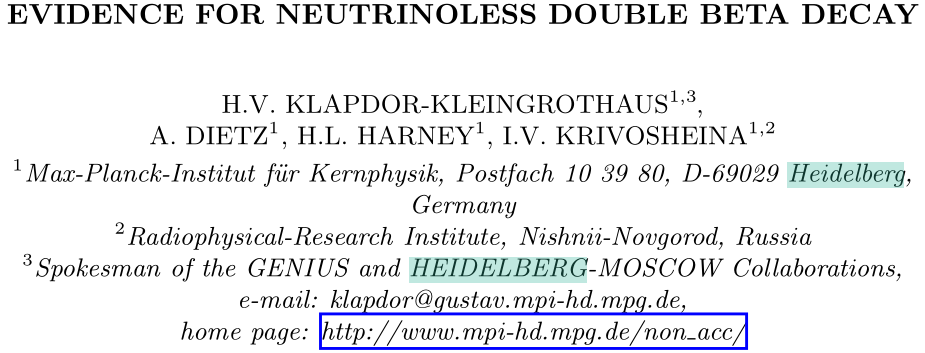
\includegraphics[width=\textwidth]{media/evidence_pic.png}
			\end{center}
		\end{subfigure}
		\begin{subfigure}[t]{.49\textwidth}
			\subcaption*{2001-03-06}
			\begin{center}
				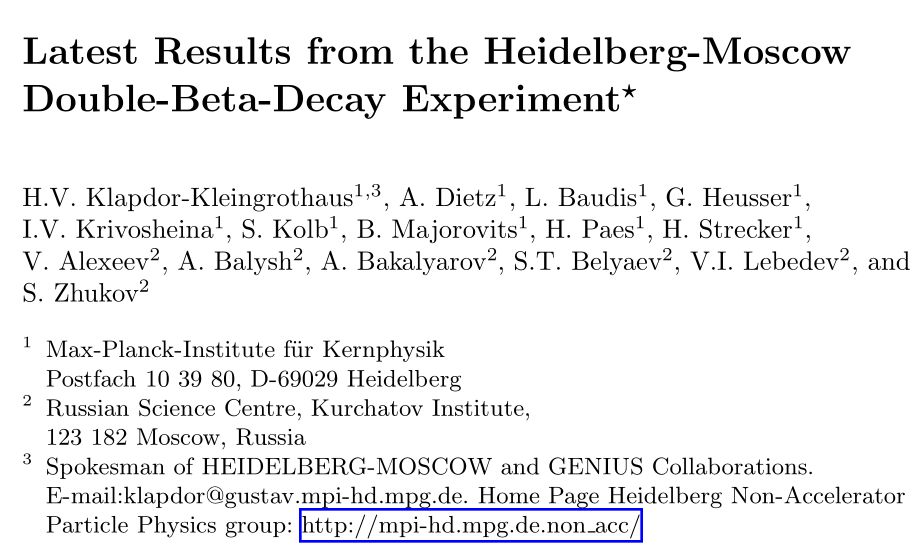
\includegraphics[width=\textwidth]{media/earlier_pic.png}
			\end{center}
		\end{subfigure}
	\end{figure}
\end{frame}
\begin{frame}{Now with $6\sigma$?}
	Klapdor-Kleingrothaus and Krivosheina published a full analysis of the HM data \footnote{\fullcite{klapdor2006evidence}} (\SI{71.7}{\kilo\gram\year})
	\begin{quote}
		\enquote{Signals near $Q_{ββ}$ are found on a 5.2σ (10.64 ± 2.06 events), 6.5σ (11.32 ±
		1.75 events) and 6.8σ (10.75 ± 1.58 events) confidence level (a, b, c, respectively).
		}
	\end{quote}
	\vspace{-1em}
	\begin{itemize}
		\item Big difference: New event selection by pulse-shape (with Neural Networks)
		\item The community generally does not believe this either
		\item \enquote{the significance varies between $2\sigma$ and $6\sigma$ being inversely proportional to the number of authors who claim it.}\footnote{\fullcite{strumia2006neutrino}}
		\item Low Event Rates $\rightarrow$ small difference in the background rate $\rightarrow$ big difference in $\sigma$\\
			$\rightarrow$ With some prevoius HM background estimations claim is less than $1\sigma$ 
	\end{itemize}
\end{frame}
